% =========================================================================== %

\begin{frame}[t,plain]
\titlepage
\end{frame}

% =========================================================================== %

\begin{frame}{Recap}
%
\begin{columns}[T]
\column{.5\linewidth}
\textbf{MatPlotLib}
\begin{itemize}
\item Befehl \texttt{plt.plot(X, Y)} und \texttt{plt.show()}
\item \texttt{plt.bar}, \texttt{plt.scatter}, \texttt{plt.quiver}, ...
\item Millionen optionale Argumente
\item Plot-Objekte \texttt{figure} und \texttt{axis}
\item Im Zweifel: Nachschlagen auf \url{https://matplotlib.org/} oder im Scrpt
\end{itemize}
%
\column{.5\linewidth}
\textbf{NumPy}
\begin{itemize}
\item Zentrales Element: \texttt{np.ndarray}
\item Komponentenweise Operationen
\item Erstellen aus Python-\texttt{list}s oder über spezielle Funktionen
\item Eigene Mathe-Bib für schnelle Operationen
\item Eigene Befehle zur Reduktion (\zB \texttt{np.sum})
\end{itemize}

\end{columns}
%
\begin{center}
	\emph{Noch Fragen?}
\end{center}
%
\end{frame}

% =========================================================================== %

\begin{frame}[fragile]
%
\begin{tcbraster}[raster columns=2,
                  raster equal height,
                  nobeforeafter,
                  raster column skip=0.5cm]
\begin{codebox}[Beispiel: Title goes here]
\begin{minted}[fontsize=\scriptsize, linenos]{python}
foo
\end{minted}
\end{codebox}
%
\begin{codebox}[Beispiel: Title goes here]
\begin{minted}[fontsize=\scriptsize, linenos]{python}
bar
\end{minted}
\end{codebox}
\end{tcbraster}
%
\end{frame}

% =========================================================================== %

\begin{frame}[fragile]{Plan für Heute}
%
\begin{itemize}
\item Etwas Physik: 
	\begin{itemize}
	\item Spin-Gitter und Magnetismus
	\item Energie
	\item Boltzmann-Verteilung
	\end{itemize}
\item Abbildung der Wirklichkeit in Code
	\begin{itemize}
	\item Liste von Eigenschaften und Fragen
	\item Auswahl geeigneter Datenstrukturen
	\item Erste Methoden
	\end{itemize}
\item Metropolis-Algorithmus
	\begin{itemize}
	\item Große Konfigurations-Räume und Monte-Carlo-Methoden
	\item Idee Metropolis für Menschen
	\item Umsetzung für den Computer
	\end{itemize}
\end{itemize}
%
\end{frame}

% =========================================================================== %

\begin{frame}{Physik: Spin-Gitter}
%
\begin{columns}[T]
\column{.5\linewidth}
\begin{itemize}
\item Vorstellung: Atome als kleine Stabmagneten
\item Drehbar im Raum
	\begin{itemize}
	\item Vereinfachung: nur zwei Möglichkeiten
	\item entweder: Nordpol \enquote{oben}
	\item oder: Nordpol \enquote{unten}
	\end{itemize}
\item Magnetfelder summieren sich auf
	\begin{itemize}
	\item Gleiche Ausrichtungen verstärken sich
	\item Gegensätze löschen sich aus
	\end{itemize}
\item Darstellung eines Festkörpers als Gitter von solchen Stabmagneten
\end{itemize}
%
\column{.5\linewidth}
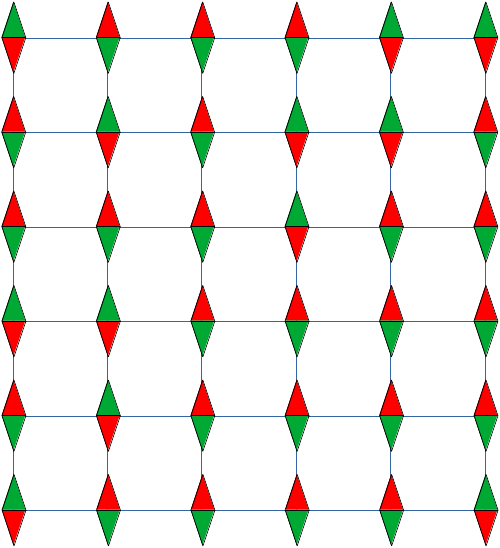
\includegraphics[width=.7\linewidth]{./gfx/spinLattice}
\end{columns}
%
\end{frame}

% =========================================================================== %\\

\begin{frame}{Physik: Gesamt-Magnetisierung und Gitter-Energie}
%
\begin{columns}[T]
\column{.5\linewidth}
\begin{itemize}
\item Gesamt-Magnetisierung
	\begin{itemize}
	\item \enquote{Wie stark ist das Magnetfeld dieses Gitters?}
	\item {}[Anzahl aller Spin-Up-Atome] minus [Anzahl aller Spin-Down-Atome]
	 \end{itemize} 
\item Gitter-Energie
	\begin{itemize}
	\item Magnete ziehen sich an oder stoßen sich ab.
	\item Es \enquote{kostet Energie}, gleichnamige Pole zueinander zu bringen
	\item Abhängig von Distanz
	\item Vereinfachung: Nur nächste Nachbarn relevant
	\end{itemize}
\end{itemize}
%
\column{.5\linewidth}
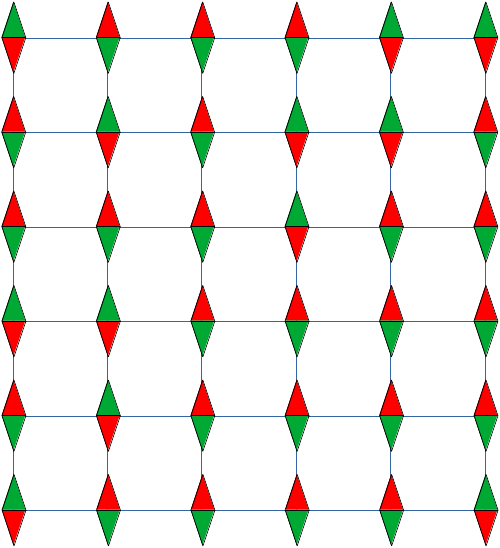
\includegraphics[width=.7\linewidth]{./gfx/spinLattice}
\end{columns}
%
\end{frame}

% =========================================================================== %\\

\begin{frame}{Physik: Magnetisierungsdichte und Gitter-Energie in Formeln}
%
\begin{itemize}
\item Stelle jeden Magneten durch Zahl dar: $+1$ oder $-1$
\item Gesamtes Gitter also durch eine Tabelle, bzw. durch Matrix $G = \left( g_{ij} \right)$
\item Magnetisierungsdichte
	\[ M = \frac{1}{V} \sum_{i, j} g_{ij} \qquad \text{mit } V: \text{\enquote{Volumen}, Anzahl Atome} \]
\item Energie
	\begin{itemize}
	\item Kopplungskonstante $J$
	\item Für jeden gleichgerichteten (\emph{parallelen}) Nachbarn: $J$ wird frei
	\item For jeden \emph{antiparallelen} Nachbarn: Energiekosten $J$ notwendig
	\item Wenn $i$ Nachbar von $j$, dann ist auch $j$ Nachbar von $i$, aber: Nur einmal Energiekosten
	\item 
		\begin{align*}
			E &= -\frac{J}{2V} \sum_x \sum_{y: y \text{ ist Nachbar von }x} g_x \cdot g_y 
			  = -\frac{J}{2V} \sum_{<x, y>} g_x \cdot g_y
		\end{align*}			
	\item Achtung: $x, y$ sind hier \emph{Koordinaten}; $x$ \enquote{enthält} also Zeilen- \emph{und} Spalten-Nummer
	\end{itemize}
\end{itemize}
%
\end{frame}

% =========================================================================== %

\begin{frame}{Physik: Erwartungswert}
%
\begin{itemize}
\item A priori: Jeder Spin frei wählbar
\item Bei $V = L \cdot L$ Gitterpunkten daher: $2^V$ Einstellungen
\item Jeweils unterschiedliche Energie
\item Nicht alle gleich wahrscheinlich!
\item Reale Welt:
	\begin{itemize}
	\item Energie eines Gegenstands unterliegt Fluktuation
	\item Daher jeder Zustand möglich
	\end{itemize}
\item Wahrscheinlichkeit hängt von der Energie ab! $p = p(E)$
\item Erwartungswert für Magnetisierung:
	\[ <M> ~ = \sum_{\text{Zustand } G} p[E(G)] \cdot M(G) \]
\end{itemize}
%
\end{frame}

% =========================================================================== %

\begin{frame}{Physik: Boltzmann-Verteilung}
%
Boltzmann-Verteilung:
\[ p(E) = \frac
	{\exp( -\frac{E}{k_B T} )}
	{\sum_\mathcal{E} \exp( -\frac{\mathcal{E}}{k_B T} )}
\]

Darin:
\begin{itemize}
\item $T$: Temperatur in Kelvin
\item $k_B$: Boltzmann-Konstante
\end{itemize}

Damit:
\begin{itemize}
\item \emph{Im Prinzip} Magnetisierung für jede Temperatur berechenbar
\item \emph{In Praxis} zu aufwändig
\end{itemize}

Ausblick:
\begin{itemize}
\item Metropolis-Algorithmus umgeht dieses Problem
\end{itemize}
%
\end{frame}

% =========================================================================== %

\begin{frame}{Programmieren: Von der Realität zum Code}
%
Wir brauchen:
\begin{itemize}
\item Vorgabe: Temperatur
\item Ein Gitter
	\begin{itemize}
	\item Bestehend aus Atomen
	\item Haben Eigenschaft \emph{Spin}: $+1$ bzw. $-1$
	\item Mit Eigenschaft: Magnetisierung
	\item Mit Eigenschaft: Gesamtenergie
	\item Beziehung \enquote{ist Nachbar von}
	\item Mit Vorgabe: Ausgangszustand
	\end{itemize}
\item Wahrscheinlichkeit, einen bestimmten Zustand eines Gitters zu realisieren
\end{itemize}
%
\end{frame}

% =========================================================================== %

\begin{frame}[fragile]{Programmieren: Ordnen und Abbilden}
%
\begin{itemize}
\item Temperatur: Erst später wichtig, wenn wir Wahrscheinlichkeiten abbilden
\item Gitter: \enquote{fühlt sich an wie ein Objekt} \Thus Klasse
	\begin{itemize}
	\item Zustand $G$: Menge aller Spins \Thus Array-Artig (\inPy{list}, NumPy-Array, ...)
		\begin{itemize}
		\item Gleichartige Informationen
		\item Ausgefüllte Tabelle
		\item[\Thus] NumPy-Array; Datentyp \texttt{np.int64}
		\item Damit implizit gegeben: \emph{Adressierung} durch Indices
		\end{itemize}
	\item \enquote{Fragen an das Gitter}: Magnetisierung und Energie
		\begin{itemize}
		\item Können aus Zustand $G$ bereichnet werden
		\item[\Thus] Methoden
		\end{itemize}
	\item Nachbarschaftsbeziehungen
		\begin{itemize}
		\item Könnten aus Koordinaten und Größe berechnet werden
		\item Aber: Werden sehr oft gebraucht
		\item Alternative: Einmal vorbereiten und Speichern
		\item Weiteres NumPy-Array
		\end{itemize}
	\end{itemize}
\end{itemize}
%
\end{frame}

% =========================================================================== %

\begin{frame}{Programmieren: Unterprobleme Auswählen}
%
\begin{itemize}
\item Wir sehen: Beschreibung \enquote{explodiert} 
	\begin{itemize}
	\item Schon einiges an Gedanken aufgeschrieben
	\item Nachbarschaftsbeziehung noch nicht fertig ausformuliert
	\item Noch gar keine Gedanken zur Darstellung der Wahrscheinlichkeit
	\end{itemize}
\item Aber: Auch schon viele konkrete Gedanken und Grundordnung
\item[\Thus] Konkreteste Ergebnisse auswählen, Rest zurückstellen
\end{itemize}
%
\end{frame}

% =========================================================================== %

\begin{frame}[fragile]{Programmieren: Klasse \texttt{Grid} -- erstes Konzept}
%
\begin{tcolorbox}[title=Klasse \texttt{Grid}]
\begin{itemize}
\item Klassenattribute
	\begin{itemize}
	\item Keine (Wenn wir mehrere Gitter im selben Programm betrachten, haben diese nichts gemeinsam)
	\end{itemize}
\item Instanzattribute
	\begin{itemize}
	\item NumPy-Array \texttt{spins}
	\item \inPy{int L}: Gitter-Breite (nicht zwingend nötig, aber \enquote{bequemer})
	\item \inPy{float J}: Kopplungs-Konstante (nötig für die Berechnung der Energie)
	\end{itemize}
\item Methoden
	\begin{itemize}
	\item \inPy{__init__(self, L, J, ??)} (vielleicht zusätzliche Parameter nötig): Bereitet ein Gitter im \emph{Ausgangszustand} vor
	\item \texttt{getMagnetization(self)} (keine weiteren Parameter)
	\item \texttt{getEnergy(self)} (keine weiteren Parameter)
	\end{itemize}
\end{itemize}
\end{tcolorbox}
%
\end{frame}

% =========================================================================== %

\begin{frame}[fragile]{Programmieren: Klasse \texttt{Grid} -- erster Code}
%
\begin{codebox}
\begin{minted}[linenos, fontsize=\scriptsize]{python3}
import numpy as np

class Grid :
    def __init__ (self, L, J = 1) :
        self.L     = L
        self.J     = J
        self.spins = np.ones(shape = (L, L), dtype=np.int64)

g = Grid(5)
print(g.spins)
\end{minted}
\end{codebox}
%
\begin{hintbox}[Offene Fragen mit einfachsten Mitteln klären]
\emph{Ausgangszustand} wurde in unseren Überlegungen bisher halb übersehen. In so einem Fall: mit einfache Fill-Ins beginnen, wie hier: \texttt{np.ones}
\end{hintbox}
%
\end{frame}

% =========================================================================== %

\begin{frame}[fragile]{Vergessene Ideen einbauen}
%
\begin{itemize}
\item Klären, was \emph{Ausgangsbedingung} heißt
	\begin{itemize}
	\item Beispiel: Wahrscheinlichkeit für einen Atom, Spin Up zu sein.
	\item[\Thus] \inPy{float}-Parameter \texttt{p} nötig: Wahrscheinlichkeit
	\end{itemize}
\item \emph{Effekte} aus dieser Erweiterung ableiten
	\begin{itemize}
	\item Spins sollen jetzt zufällig sein
	\item[\Thus] keine neuen Attribute nötig
	\item[\Thus] \texttt{np.ones} (alleine) reicht dafür nicht mehr
	\end{itemize}
\item Effekt als neue Methode einbauen
	\begin{itemize}
	\item Aufgaben, die von einer Methode erfüllt werden sollten sehr übersichtlich bleiben
	\item \enquote{Ein Gedanke -- eine Aufgabe}. Selten mehr als 20 Zeilen pro Funktion/Methode
	\item Neue Methode: Suche zufällige Atome aus und drehe deren Spin
	\end{itemize}
\end{itemize}
%
\end{frame}

% =========================================================================== %

\begin{frame}[fragile]
%
\begin{codebox}
\begin{minted}[linenos, fontsize=\scriptsize]{python3}
import numpy as np

class Grid :
    def __init__ (self, L, J = 1, p = None) :
        self.L     = L
        self.J     = J
        self.spins = np.ones(shape = (L, L), dtype=np.int64)
        
        if p : self.shake(p)
        
    def shake (self, p = 0.5) :
        mask = np.random.uniform(size = (self.L, self.L)) < p
        self.spins[mask] *= -1

g = Grid(5, 1, 0.5)
print(g.spins)
\end{minted}
\end{codebox}
%
\end{frame}

% =========================================================================== %

\begin{frame}[fragile]{Methoden anbauen}
%
\begin{tcbraster}[raster columns=2,
                  raster equal height,
                  nobeforeafter,
                  raster column skip=0.5cm]
\begin{codebox}[Erste geplante Methode]
\begin{minted}[linenos, fontsize=\scriptsize]{python3}
import numpy as np

class Grid :
    # wie zuvor
    
    def magnetization (self) :
        return np.sum(self.spins) / \
               self.L ** 2
    
    def energy (self) :
        # ???
        pass

g = Grid(5, 1, 0.5)
print(g.spins)
print(g.magnetization())
\end{minted}
\end{codebox}
%
\begin{cmdbox}[Ausgabe]
\begin{minted}[fontsize=\scriptsize]{text}

[[ 1 -1  1 -1 -1]
 [-1  1  1 -1 -1]
 [ 1  1  1 -1  1]
 [ 1  1 -1 -1  1]
 [-1 -1 -1 -1 -1]]
-0.12
\end{minted}
\end{cmdbox}
\end{tcbraster}
%
\end{frame}

% =========================================================================== %

\begin{frame}[fragile]{Nachbarschaftslisten}
%
\begin{itemize}
\item Schon angesprochen: Speicherplatz für Rechenzeit opfern
\item Selbe Denkansätze
	\begin{itemize}
	\item Liste von Koordinaten
	\item Immer gleicher Datentyp, vollständig ausgefüllte Tabelle
	\item[\Thus] NumPy-Array
	\item \enquote{Tabelle mit \inPy{tuple}s als Einträgen} (4 Nachbarn mit je Zeile und Spalte)
	\end{itemize}
\item Im Code einpflegen...
	\begin{itemize}
	\item ... als eigene Methode ...
	\item ... die von \inPy{__init__} aufgerufen wird
	\end{itemize}
\item Sonderfall: Am Rand?
	\begin{itemize}
	\item Verschiedene Ansätze denkbar
	\item Häufig, weil einfach: \emph{zyklische Randbedingungen}: linker Rand benachbart mit rechtem Rand, oberer Rand mit unterem Rand
	\item Alternativ auch: Einträge leer lassen
	\end{itemize}
\end{itemize}
%
\end{frame}

% =========================================================================== %

\begin{frame}[fragile]
%
\begin{codebox}
\begin{minted}[linenos, fontsize=\scriptsize]{python3}
class Grid :
    def __init__ (self, L, J = 1, p = None) :
        self.L          = L
        self.J          = J
        self.spins      = np.ones (shape = (L, L)   , dtype = np.int64)
        self.neighbours = np.zeros(shape = (L, L, 4, 2), dtype = np.int64)
        self.makeNeighbourList()
        if p : self.shake(p)
    
    def makeNeighbourList (self) :
        for     row in range(self.L) :
            for col in range(self.L) :
                self.neighbours[row][col][0] = (row - 1, col    )
                self.neighbours[row][col][1] = (row + 1, col    )
                self.neighbours[row][col][2] = (row    , col - 1)
                self.neighbours[row][col][3] = (row    , col + 1)
                
        mask = self.neighbours < 0
        self.neighbours[mask]  += self.L
        mask = self.neighbours >= self.L
        self.neighbours[mask]  -= self.L
\end{minted}
\end{codebox}
%
\end{frame}

% =========================================================================== %

\begin{frame}[fragile]{Optimierung}
%
\begin{itemize}
\item Symmetrie der Nachbarschaftsbeziehung
\item Statt: Jeden Nachbarn halb zu zählen: nur die hälfte der Nachbarn zählen!
\end{itemize}
%
\begin{codebox}
\begin{minted}[linenos, fontsize=\scriptsize]{python3}
class Grid :
    def __init__ (self, L, J = 1, p = None) :
        # ...
        self.neighbours = np.zeros(shape = (L, L, 2, 2), dtype = np.int64)
        # ...
    
    def makeNeighbourList (self) :
        for     row in range(self.L) :
            for col in range(self.L) :
                self.neighbours[row][col][1] = (row + 1, col    )
                self.neighbours[row][col][3] = (row    , col + 1)
                
        mask = self.neighbours >= self.L
        self.neighbours[mask]  -= self.L
\end{minted}
\end{codebox}
%
\end{frame}

% =========================================================================== %

\begin{frame}[fragile]
%
\begin{codebox}
\begin{minted}[linenos, fontsize=\scriptsize]{python3}
class Grid :
    # ...
    
    def energy (self) :
        reVal = 0
        
        for     row in range(self.L) :
            for col in range(self.L) :
                neighbours = self.neighbours[row, col]
                for neighbour in neighbours :
                    reVal += self.spins[row, col] * self.spins[tuple(neighbour)]
        
        return reVal / self.L ** 2

g = Grid(5, 1, 0)           # für Wahrscheinlichkeit 0 kann das Ergebnis 
print(g.spins)              # besonders leicht vorhergesagt werden!

print("mag:", g.magnetization())
print(" E :", g.energy())
\end{minted}
\end{codebox}
%
\end{frame}

% =========================================================================== %

\begin{frame}{Methode und Aufwand}
%
\begin{itemize}
\item Jetzt theoretisch möglich:
	\begin{itemize}
	\item Für jede Gitter-Konfiguration Energie und Wahrscheinlichkeit berechnen
	\item Daraus schließlich Erwartungswert für Magnetisierung berechnen
	\end{itemize}
\item Anzahl Gitter-Konfigurationen: $2^V$
	\begin{itemize}
	\item Für unser \emph{winziges} Gitter mit 25 Atomen: Bereits 33\,554\,432 Anordnungen.
	\item Annahme: Rechenzeit pro Anordnung \SI{1}{ms}
	\item[\Thus] 9 Stunden 19 Minuten
	\item[\Thus]  \emph{Dickes Uff}
	\end{itemize}
\end{itemize}
%
\end{frame}

% =========================================================================== %

\begin{frame}{Lösung: Monte-Carlo-Methoden}
%
\begin{itemize}
\item \emph{Zufällige} Konfigurationen auswählen
\item[\Thus] Statt gesamten Konfigurationsraum zu erforschen: Stichproben
\item Vergleiche: Wahlprognose bei Bundestagswahl
	\begin{itemize}
	\item Stichprobe muss repräsentativ sein
	\item \enquote{muss der richtigen Wahrscheinlichkeitsverteilung folgen}
	\item Bei Gleichverteilung: Zufällig ziehen reicht.
	\end{itemize}
\item Einige \enquote{mathematische Tricks} garantieren Boltzmann-Verteilung
\item[\Thus] \emph{Metropolis-Algorithmus}
\end{itemize}
%
\end{frame}

% =========================================================================== %

\begin{frame}{Metropolis-Algorithmus für Menschen}
%
\begin{itemize}
\item Wähle zufälliges Atom aus
\item Berechne, wie sich Gitter-Energie ändert, wenn Spin gedreht wird.
	\begin{itemize}
	\item Wenn Energie sinkt: mache diese Änderung auf jeden Fall
	\item Wenn Energie steigt: mache diese Änderung mit $p = \exp(-\frac{\Delta E}{k_B T})$
	\end{itemize}
\item Speichere die entstehende Konfiguration (auch, wenn keine Änderung stattfand)
\item Wiederhole dies oft
\item[\Thus] Erhalte \enquote{Liste von Konfigurationen} $G_1, G_2, ... G_N$
	\begin{itemize}
	\item Konfigurationen in dieser Liste sind Boltzmann-Verteilt
	\item Ein Durchschnitt über Messgrößen an diesen Konfigurationen gibt auch den Erwartungswert der Messgröße selbst.
	\item \zB: Erhalte $M(G_1), M(G_2), ...$ und bilde Durchschnittt $<M>$. Dieser nähert sich dem \enquote{exakten} Erwartungswert an
	\end{itemize}
\end{itemize}
%
\end{frame}

% =========================================================================== %

\begin{frame}{Umsetzung für den Computer}
%
\begin{center}
(Datei \texttt{007-Ising-f.py})
\end{center}
%
\end{frame}

% =========================================================================== %

\begin{frame}{Disclaimer und Werbung}
%
\begin{hintbox}[Vorlesung \emph{Monte Carlo Methods for Physicists}]
Der gezeigte Code ist noch lange nicht optimal. Ich wollte hier nicht zu sehr in Details einsteigen, die in einer anderen Vorlesung ohnehin ausführlicher behandelt werden. Was ich hier ausgelassen habe sind aber im Wesentlichen nur Aufbauten auf das Schema in dieser Vorlesung.

Bei mehr Interesse kann ich (NaturwissenschaflterInnen) die Vorlesung \emph{Monte Carlo Methods for Physicists} bei Prof. Bloch sehr empfehlen. Neben dem Ising-Modell werden auch Erweiterungen und fortgeschrittene Algorithmen besprochen.
\end{hintbox}
%
\end{frame}
